\section{Measurement task}
\textbf{Define a set of measurements or markups that would enable a hypothetical medical expert to gain insights into the volumetric model used in Task 1}\\

For the lungs segmentation. The following markups could be of interest in order to monitor lung progression for smokers along time.

\begin{itemize}
    \item \textbf{Lung Perimeter:} Measure the total volume of each lung to monitor changes over time, which could indicate disease progression or improvement.
    \item \textbf{Nodule Height:} Place fiducial markers on any detected nodules within the lungs to measure their size and track growth or shrinkage over time.
    \item \textbf{Airway Width:} Use line markups to measure the diameter of major airways (e.g., trachea, bronchi) to assess for any narrowing or obstruction.
\end{itemize}

\begin{figure}[H]
    \centering
    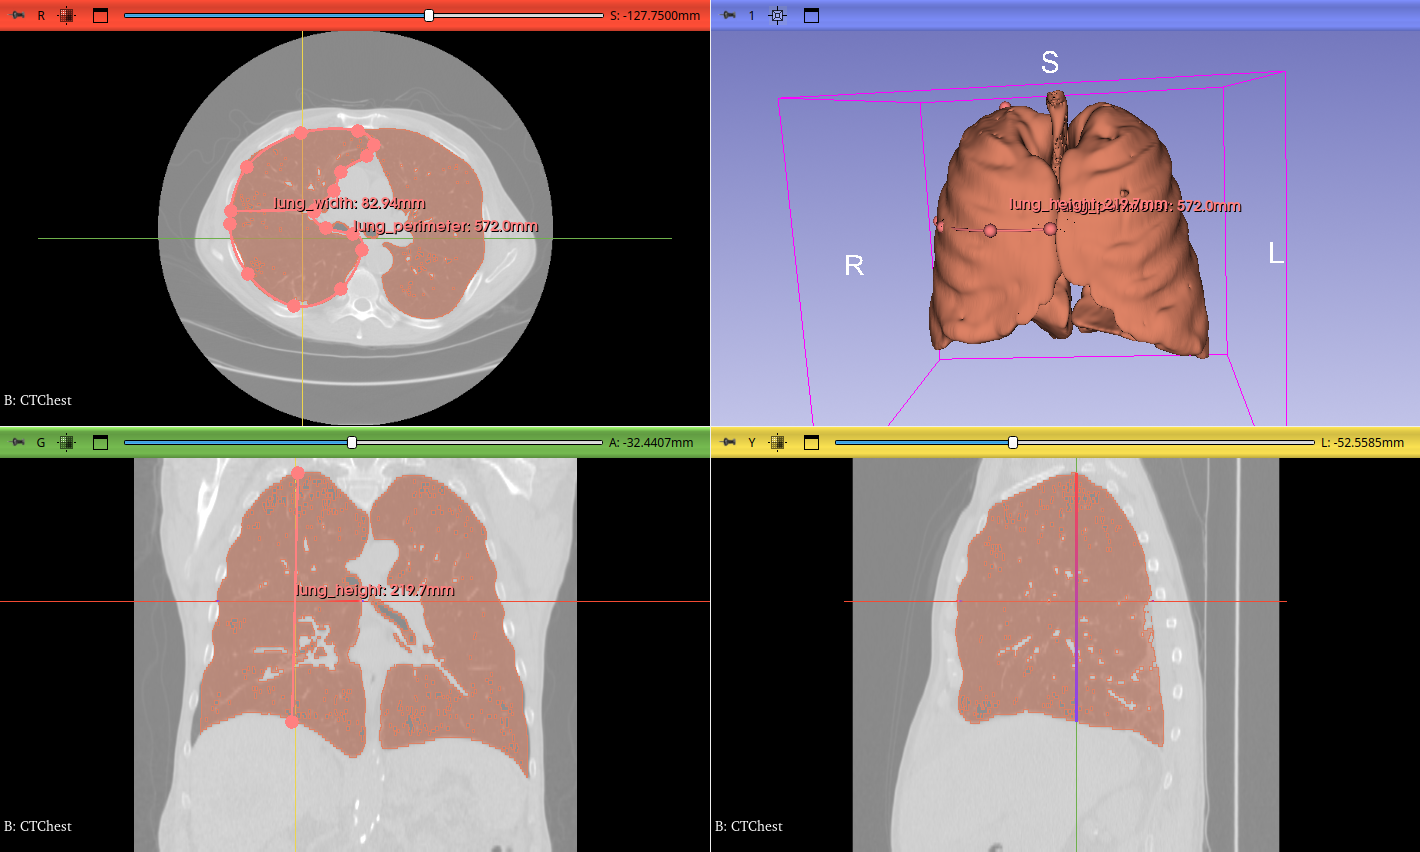
\includegraphics[width=0.7\textwidth]{img/ex31.png}
    \caption{Visualization of the lungs segmentation with fiducial markers on detected nodules and line markups on airways.}
    \label{fig:lung_measurements}
\end{figure}


Those metrics have been obtained with the markups module. The following results were obtained:

\begin{table}[H]
    \centering
    \begin{tabular}{|c|c|}
        \hline
        \textbf{Measurement} & \textbf{Value} \\
        \hline
        Lung Perimeter & 572.0 mm \\
        Lung Height & 219.7 mm \\
        Lung Width & 82.9 mm \\
        \hline
    \end{tabular}
    \caption{Lung measurements obtained from the segmentation model.}
    \label{tab:lung_measurements}
\end{table}


